\section{Overlays}
\subsection{Incremental lists}

\begin{frame}[label=overlays]{Incremental lists}
  \begin{itemize}[<+-| alert@+>]
    \item First, each item appears and is highlighted while it is new
    \item Then the next one takes over
    \item Specs like \texttt{<+-| alert@+>} work on whole lists
  \end{itemize}
  \pause
  \begin{enumerate}[(a)]
    \item<5-> custom enumerate labels
    \item<6-> with explicit overlays \only<6>{(only on step 6)}
  \end{enumerate}
\end{frame}

\begin{frame}{Swapping content with \texttt{\textbackslash only} and \texttt{overprint}}
  \begin{columns}[T]
    \column{0.48\textwidth}
      \only<1>{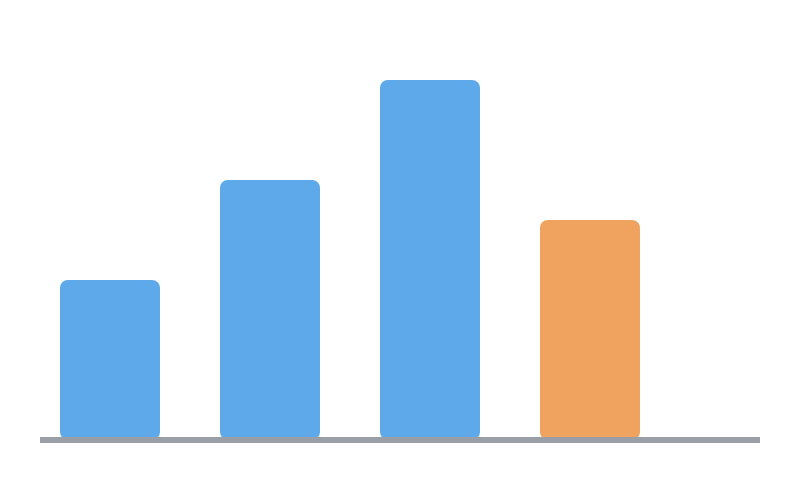
\includegraphics[width=0.9\linewidth]{bars}}
      \only<2->{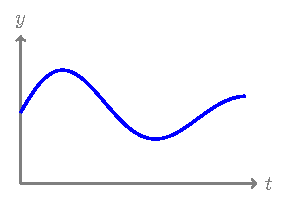
\includegraphics[width=0.9\linewidth]{diagram}}
      \centering
      \alt<1>{A bar chart (PNG)}{A damped wave (PDF)}
    \column{0.48\textwidth}
      \begin{overprint}
        \onslide<1>
          \begin{block}{Step one}
            The left figure is a PNG file.
          \end{block}
        \onslide<2>
          \begin{alertblock}{Step two}
            Now it is a PDF, rasterised at build time.
          \end{alertblock}
        \onslide<3>
          \begin{exampleblock}{Step three}
            \texttt{overprint} reserves room for its tallest part.
          \end{exampleblock}
      \end{overprint}
  \end{columns}
\end{frame}

\begin{frame}{Covered items and bare \texttt{\textbackslash onslide}}
  With \texttt{\textbackslash setbeamercovered\{transparent\}}, future content shows faintly:
  \begin{itemize}
    \item<1-> Always here
    \item<2-> From step two, \textbf<3>{bold on step three}
    \item<3-> From step three
  \end{itemize}
  \onslide<4->
  A paragraph uncovered by a bare \texttt{\textbackslash onslide<4->} switch.
\end{frame}

\begin{frame}{TikZ with overlays}
  \begin{center}
  \begin{tikzpicture}[scale=1.4]
    \draw[->] (0,0) -- (5,0) node[right] {$x$};
    \draw[->] (0,0) -- (0,3) node[above] {$f(x)$};
    \pause
    \draw[blue, very thick] (0.2,2.6) .. controls (1.5,-0.5) and (3.5,-0.5) .. (4.8,2.6);
    \pause
    \fill[orange] (2.5,0.35) circle (3pt) node[below=4pt] {$x^\ast$};
  \end{tikzpicture}
  \end{center}
\end{frame}
